\subsection{Experimental Setup}
\label{sec:setup}

\subsubsection{System used}

Experiments are performed on a system featuring an NVIDIA A100 GPU with $108$ SMs and $64$ CUDA cores per SM. The GPU has $80$ GB of global memory, with a bandwidth of $1935$ GB/s. Each SM has a shared memory capacity of $164$ KB. The system also has an AMD EPYC-7742 processor with $64$ cores, running at a frequency of $2.25$ GHz.\ignore{Each core has $4$ MB L1 cache, a $32$ MB L2 cache, and shares a $256$ MB L3 cache.} The server is set up with $512$ GB of DDR4 system memory and runs Ubuntu $20.04$.


\subsubsection{Configuration}

We utilize 32-bit integers to represent vertex IDs and 64-bit floating-point numbers for vertex ranks. Affected vertices are denoted by an 8-bit integer vector. Our configuration sets the damping factor to $\alpha = 0.85$ \cite{rank-langville06}, the frontier tolerance $\tau_f$ to $10^{-6}$ \cite{sahu2024df}, the prune tolerance $\tau_p$ to $10^{-6}$ \cite{sahu2024df}, and the iteration tolerance $\tau$ to $10^{-10}$ using the $L_\infty$-norm \cite{rank-dubey22, rank-plimpton11}. We cap the maximum number of iterations $MAX\_ITERATIONS$ at $500$ \cite{nvgraph}. Compilation is performed using NVCC, a part of CUDA toolkit $11.4$, and OpenMP $5.0$ (for CPU code). OpenMP's \textit{dynamic schedule} with a chunk size of $2048$ is used for CPU-based computations to facilitate dynamic workload balancing among threads.


\subsubsection{Dataset}
\label{sec:dataset}

To experiment with real-world dynamic graphs, we employ five temporal networks sourced from the Stanford Large Network Dataset Collection \cite{snapnets}. Details of these graphs are summarized in Table \ref{tab:dataset}. Here, the number of vertices range from $24.8$ thousand to $2.60$ million, temporal edges from $507$ thousand to $63.4$ million, and static edges from $240$ thousand to $36.2$ million. For investigations involving large static graphs with random batch updates, we utilize $12$ graphs as listed in Table \ref{tab:dataset}, obtained from the SuiteSparse Matrix Collection \cite{suite19}. Here, the number of vertices range from $3.07$ to $214$ million, and edges from $25.4$ million to $3.80$ billion. To mitigate dead ends (vertices without out-links) and the associated overhead of global teleport rank computation in each iteration, we augment all vertices with self-loops\ignore{within the graph} \cite{kolda2009generalized, rank-andersen07, rank-langville06}.

\begin{table}[hbtp]
  \centering
  \caption{List of 5 real-world dynamic graphs\ignore{, i.e., temporal networks}, obtained from the Stanford Large Network Dataset Collection \cite{snapnets}. Here, $|V|$ is the number of vertices, $|E_T|$ the number of temporal edges\ignore{(includes duplicate edges)}, and $|E|$ the number of static edges (with no duplicates).\ignore{, and $\Gamma_G$ is the Gini coefficient of PageRank distribution. In the table, B refers to a billion, M refers to a million and K refers a thousand.}}
  \label{tab:dataset}
  \begin{tabular}{|c||c|c|c|c|}
    \toprule
    \textbf{Graph} &
    \textbf{\textbf{$|V|$}} &
    \textbf{\textbf{$|E_T|$}} &
    \textbf{\textbf{$|E|$}} \\
    \midrule
    sx-mathoverflow & 24.8K & 507K & 240K \\ \hline
    sx-askubuntu & 159K & 964K & 597K \\ \hline
    sx-superuser & 194K & 1.44M & 925K \\ \hline
    wiki-talk-temporal & 1.14M & 7.83M & 3.31M \\ \hline
    sx-stackoverflow & 2.60M & 63.4M & 36.2M \\ \hline
  \bottomrule
  \end{tabular}
\end{table}

\begin{table}[hbtp]
  \centering
  \caption{List of $12$ graphs sourced from the SuiteSparse Matrix Collection \cite{suite19}, where directed graphs are indicated with $*$. Here, $|V|$ denotes the number of vertices, $|E|$ represents the number of edges (inclusive of self-loops), and $D_{avg}$ represents the average degree.}
  \label{tab:dataset-large}
  \begin{tabular}{|c||c|c|c|c|}
    \toprule
    \textbf{Graph} &
    \textbf{\textbf{$|V|$}} &
    \textbf{\textbf{$|E|$}} &
    \textbf{\textbf{$D_{avg}$}} \\
    \midrule
    \multicolumn{4}{|c|}{\textbf{Web Graphs (LAW)}} \\ \hline
    indochina-2004$^*$ & 7.41M & 199M & 26.8 \\ \hline  % & \num{4.7e-4}
    % uk-2002$^*$ & 18.5M & 311M & 16.8 \\ \hline  % & \num{9.6e-5}
    arabic-2005$^*$ & 22.7M & 654M & 28.8 \\ \hline  % & \num{5.5e-4}
    uk-2005$^*$ & 39.5M & 961M & 24.3 \\ \hline  % & \num{9.6e-5}
    webbase-2001$^*$ & 118M & 1.11B & 9.4 \\ \hline  % & \num{7.3e-7}
    it-2004$^*$ & 41.3M & 1.18B & 28.5 \\ \hline  % & \num{3.8e-4}
    sk-2005$^*$ & 50.6M & 1.98B & 39.1 \\ \hline  % & \num{5.8e-4}
    \multicolumn{4}{|c|}{\textbf{Social Networks (SNAP)}} \\ \hline
    com-LiveJournal & 4.00M & 73.4M & 18.3 \\ \hline  % & \num{7.9e-4}
    com-Orkut & 3.07M & 237M & 77.3 \\ \hline  % & \num{6.7e-2}
    \multicolumn{4}{|c|}{\textbf{Road Networks (DIMACS10)}} \\ \hline
    asia\_osm & 12.0M & 37.4M & 3.1 \\ \hline  % & \num{8.4e-4}
    europe\_osm & 50.9M & 159M & 3.1 \\ \hline  % & \num{6.6e-4}
    \multicolumn{4}{|c|}{\textbf{Protein k-mer Graphs (GenBank)}} \\ \hline
    kmer\_A2a & 171M & 531M & 3.1 \\ \hline  % & \num{9.4e-5}
    kmer\_V1r & 214M & 679M & 3.2 \\ \hline  % & \num{3.2e-4}
  \bottomrule
  \end{tabular}
\end{table}



\subsubsection{Batch Generation}
\label{sec:batch-generation}

For experiments involving real-world dynamic graphs, we first load $90\%$ of each graph from Table \ref{tab:dataset}, and add self-loops to all vertices. Subsequently, we load $B$ edges in $100$ batch updates. Here, $B$ denotes the desired batch size, specified as a fraction of the total number of temporal edges $|E_T|$ in the graph.\ignore{Additionally, self-loops are added to all vertices with each batch update.} For experiments on large graphs with random batch updates, we select each base (static) graph from Table \ref{tab:dataset-large} and generate a random batch update comprising an $80\% : 20\%$ mix of edge insertions and deletions to emulate realistic batch updates. To prepare the set of edges for insertion, we select vertex pairs with equal probability. For edge deletions, we uniformly delete each existing edge. To simplify, we ensure no new vertices are added or removed from the graph. The batch size is measured as a fraction of edges in the original graph, ranging from $10^{-7}$ to $0.1$ (i.e., $10^{-7}|E|$ to $0.1|E|$), with multiple batches generated for each size for averaging. Self-loops are added to all vertices alongside each batch update, as\ignore{mentioned} earlier.


\subsubsection{Measurement}
\label{sec:measurement}

We assess the runtime of each approach on the entire updated graph, including partitioning, initial marking of affected vertices, and convergence detection time. However, we exclude the time taken for memory transfers (to and from the GPU) as well as allocation/deallocation. The mean time and error for a specific method at a given batch size are computed as the geometric mean across input graphs. Additionally, we evaluate the error/accuracy of each approach by measuring the $L1$-norm \cite{ohsaka2015efficient} of the returned ranks compared to ranks obtained from a reference Static PageRank run on the updated graph with an extremely low iteration tolerance of $\tau = 10^{-100}$, limited to $500$ iterations.




\subsection{Performance of Our Static PageRank}
\label{sec:static-comparison}

\begin{figure*}[hbtp]
  \centering
  \subfigure[Runtime in seconds (logarithmic scale) with \textit{Hornet}, \textit{Gunrock}, \textit{Our} Static PageRank.]{
    \label{fig:compare--runtime}
    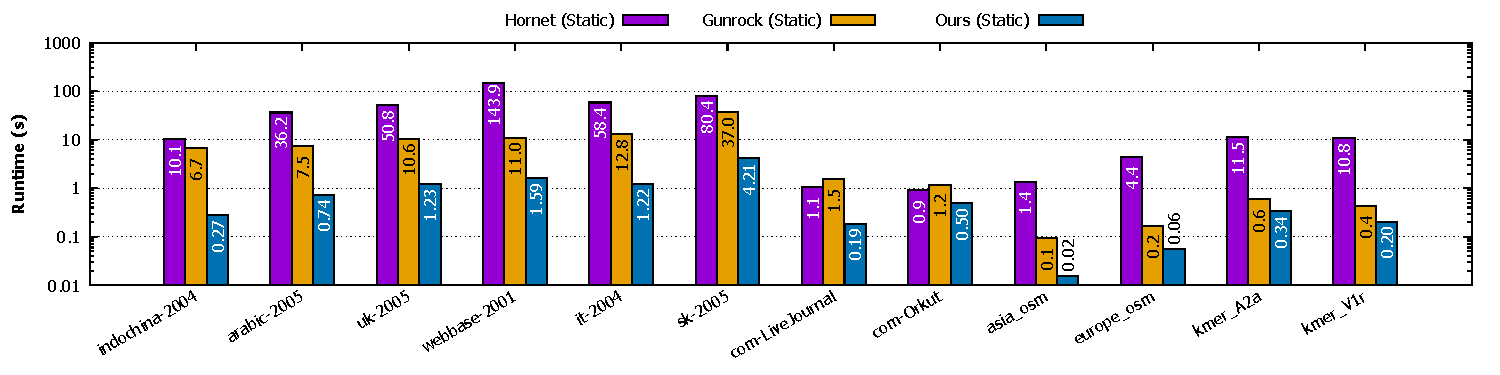
\includegraphics[width=0.98\linewidth]{out/compare-runtime.pdf}
  } \\[-0ex]
  \subfigure[Speedup of \textit{Our} Static PageRank (logarithmic scale) with respect to \textit{Hornet} and \textit{Gunrock}.]{
    \label{fig:compare--speedup}
    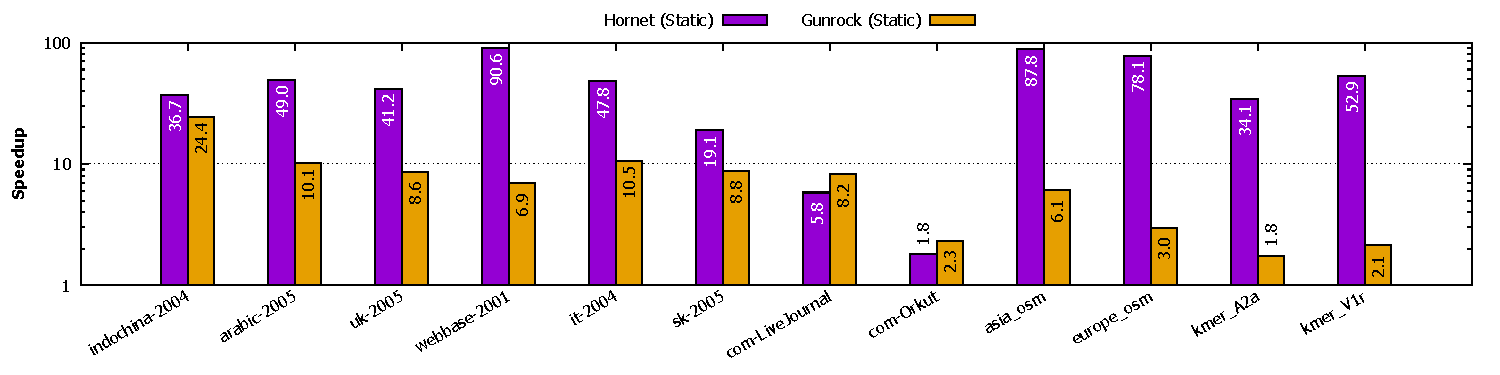
\includegraphics[width=0.98\linewidth]{out/compare-speedup.pdf}
  } \\[-2ex]
  \caption{Runtime in seconds and speedup (log-scale) with \textit{Hornet}, \textit{Gunrock}, \textit{Our} Static PageRank for each graph in the dataset.}
  \label{fig:compare}
\end{figure*}


We now evaluate the performance of our GPU implementation of Static PageRank, and compare it with the performance of Static PageRank in the Hornet \cite{busato2018hornet} and Gunrock \cite{wang2016gunrock} graph processing frameworks on large (static) graphs from Table \ref{tab:dataset-large}. For Hornet, we use a CUDA C++ program to read each input graph with \texttt{GraphStd::re} \texttt{ad()}, perform \texttt{HornetInit}, create a \texttt{HornetGraph}, and set up \texttt{Stati} \texttt{cPageRank} with a damping factor $\alpha$ of $0.85$, and iteration tolerance $\tau$ of $10^{-10}$, and limit the maximum number of iterations to $500$. We also define a new PageRank operator called \texttt{Max}, to compute $L_\infty$-norm of the absolute difference between the previous and current rank vectors (since we use $L_\infty$-norm for convergence detection), and use this for convergence detection (with \texttt{forAllnumV()}) instead of $L1$-norm (used by default). To perform the PageRank computation, we then use \texttt{StaticPageRank::run()}, and measure its runtime with \texttt{Timer<DEVICE>}. For Gunrock, we use a CUDA C++ program to read each input graph in Table \ref{tab:dataset-large} with \texttt{io::matrix\_market\_t::load()}, convert it to a CSR representation with \texttt{format::csr\_t::from\_coo()}, and build a graph with \texttt{graph::build::from\_csr()}. We then perform PageRank computation with \texttt{gunrock::pr::run()} upon the loaded graph with a damping factor $\alpha$ of $0.85$, an iteration tolerance of $10^{-10}$, and limit the number of iterations to $500$ by modifying the \texttt{gunrock::pr::en} \texttt{actor\_t::is\_} \texttt{converged()} function (note that Gunrock uses $L_\infty$-norm for convergence detection by default), and record the runtime reported by \texttt{gunrock::pr::run()}.\ignore{Neither Hornet nor Gunrock offer GPU implementation of dynamic PageRank algorithms.}

Figure \ref{fig:compare--runtime} illustrates the runtime of Hornet, Gunrock, and our Static PageRank on the GPU, for each graph in the dataset. On the \textit{sk-2005} graph, our Static PageRank computes the ranks of vertices with an iteration tolerance $\tau$ of $10^{-10}$ in $4.2$ seconds, achieving a processing rate of $471$ million edges/s. Figure \ref{fig:compare--speedup} shows the speedup of Our Static PageRank with respect to Hornet and Gunrock. Our Static PageRank is on average $31\times$ faster than Hornet, and $5.9\times$ times faster than Gunrock. This speedup is particularly high on the \textit{webbase-2001} graph and road networks with Hornet, and on the \textit{indochina-2004} graph with Gunrock. Further, our GPU implementation of Static PageRank is on average $24\times$ times faster than our parallel multicore implementation of Static PageRank.




\subsection{Performance of Our DF-P PageRank}

\subsubsection{Results on real-world dynamic graphs}

We now compare the performance of our GPU implementation of Dynamic Frontier (DF) and Dynamic Frontier with Pruning (DF-P) PageRank with Static, Naive-dynamic (ND), and Dynamic Traversal (DT) PageRank on real-world dynamic graphs from Table \ref{tab:dataset}. This is done on batch updates of size $10^{-5}|E_T|$ to $10^{-3}|E_T|$ in multiples of $10$. For each batch size, as mentioned in Section \ref{sec:batch-generation}, we load $90\%$ of the graph, add self-loops to all vertices in the graph, and then load $B$ edges (where $B$ is the batch size) consecutively in $100$ batch updates. Figure \ref{fig:temporal-summary--runtime-overall} displays the overall runtime of each approach across all graphs for each batch size, while Figure \ref{fig:temporal-summary--error-overall} illustrates the overall rank error compared to a reference Static PageRank run (as described in Section \ref{sec:measurement}). Additionally, Figures \ref{fig:temporal-summary--runtime-graph} and \ref{fig:temporal-summary--error-graph} present the mean runtime and rank error of the approaches on each dynamic graph in the dataset. Figure \ref{fig:temporal-compare} presents a comparison of the overall runtime and error between the GPU implementation of each approach and its respective CPU counterpart. Finally, Figures \ref{fig:temporal-sx-mathoverflow}, \ref{fig:temporal-sx-askubuntu}, \ref{fig:temporal-sx-superuser}, \ref{fig:temporal-wiki-talk-temporal}, and \ref{fig:temporal-sx-stackoverflow} show the runtime and rank error of the approaches on each dynamic graph in Table \ref{tab:dataset}, upon each consecutive batch update.

\begin{figure*}[!hbt]
  \centering
  \subfigure[Overall Runtime]{
    \label{fig:temporal-summary--runtime-overall}
    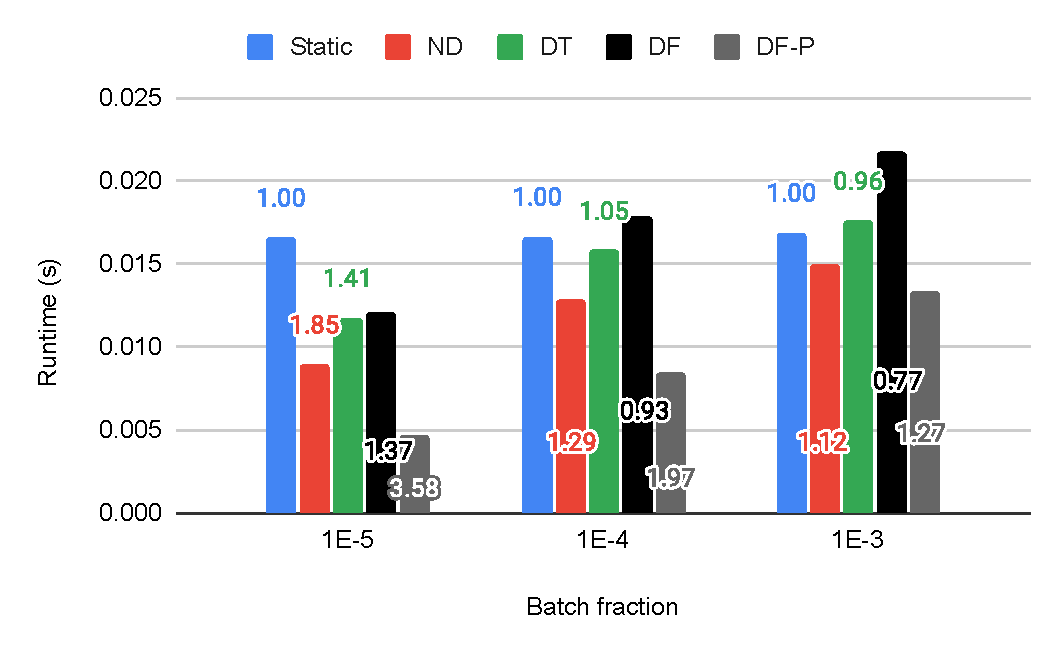
\includegraphics[width=0.48\linewidth]{out/temporal-summary-runtime-overall.pdf}
  }
  \subfigure[Overall Error in ranks obtained]{
    \label{fig:temporal-summary--error-overall}
    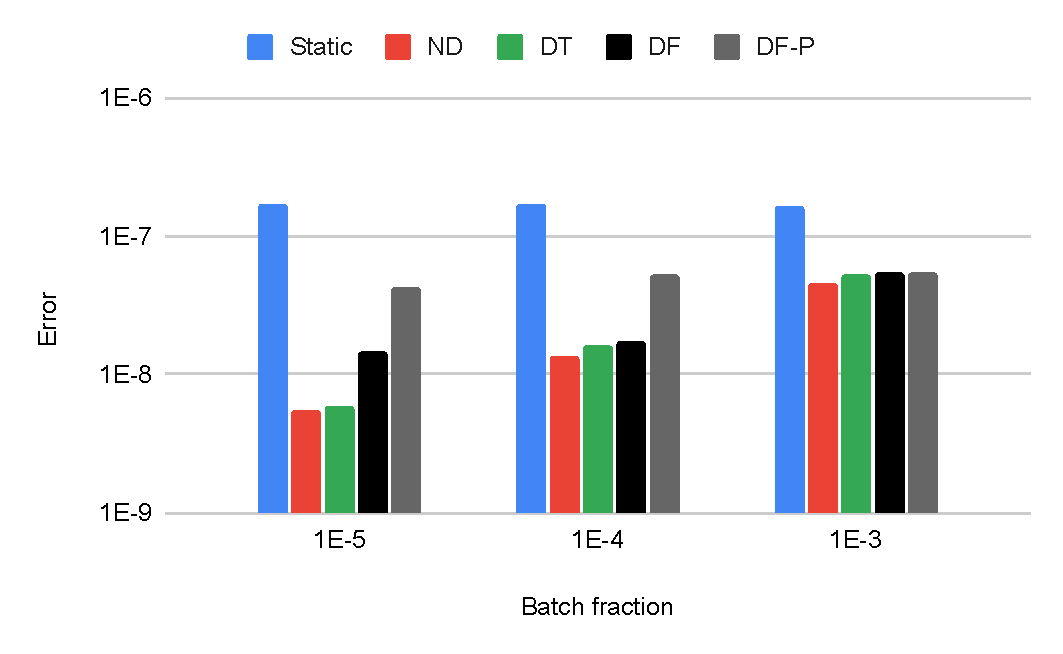
\includegraphics[width=0.48\linewidth]{out/temporal-summary-error-overall.pdf}
  } \\[2ex]
  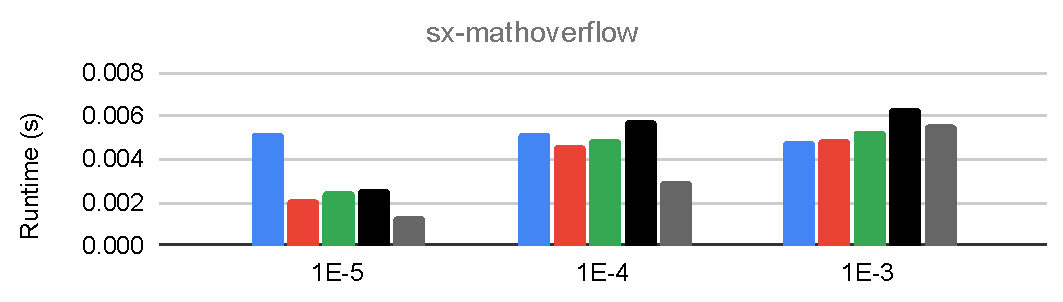
\includegraphics[width=0.48\linewidth]{out/temporal-summary-runtime-sx-mathoverflow.pdf}
  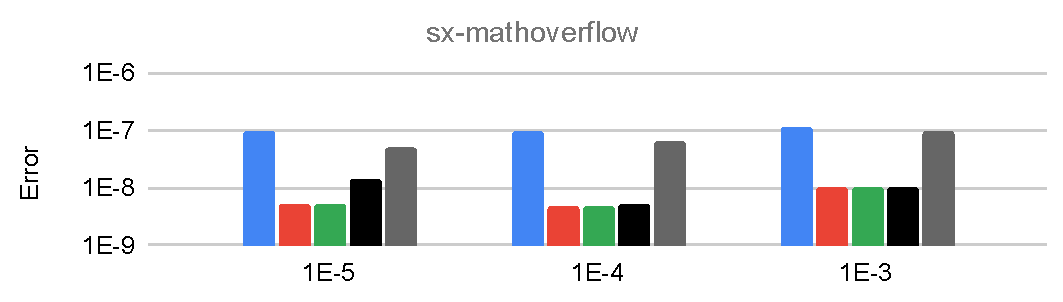
\includegraphics[width=0.48\linewidth]{out/temporal-summary-error-sx-mathoverflow.pdf}
  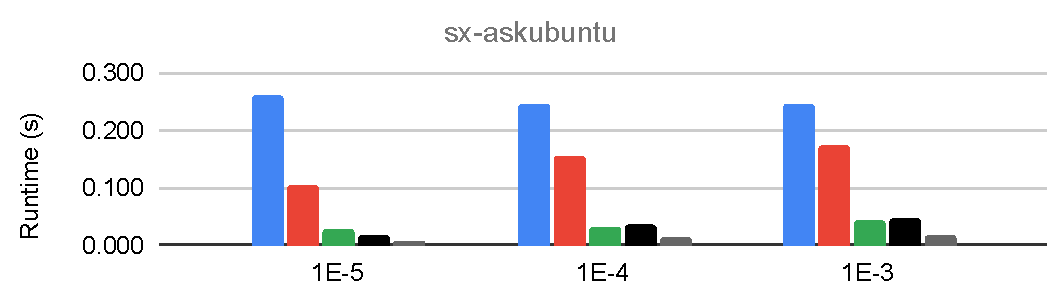
\includegraphics[width=0.48\linewidth]{out/temporal-summary-runtime-sx-askubuntu.pdf}
  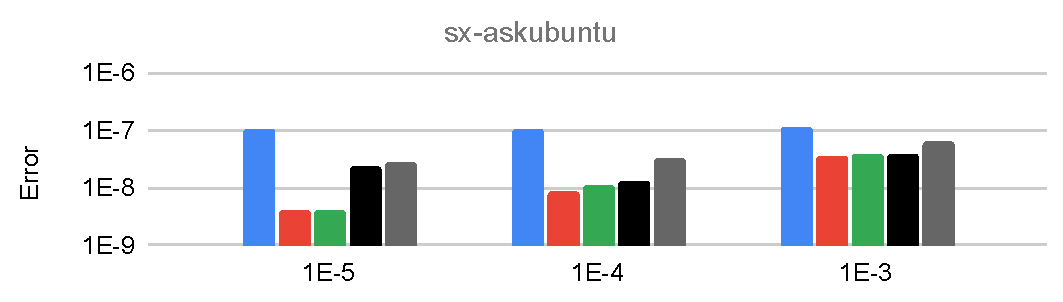
\includegraphics[width=0.48\linewidth]{out/temporal-summary-error-sx-askubuntu.pdf}
  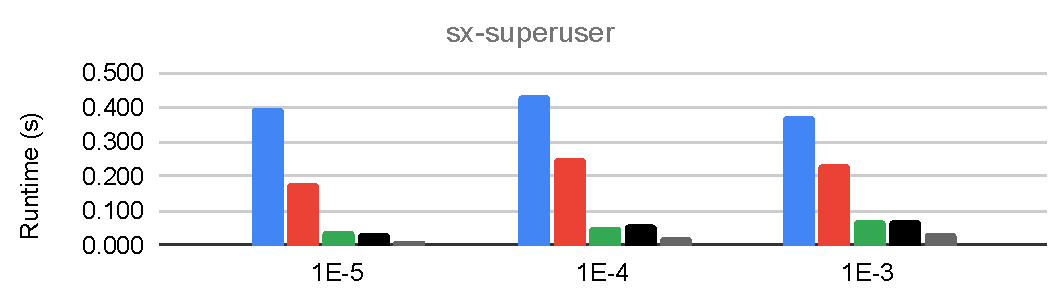
\includegraphics[width=0.48\linewidth]{out/temporal-summary-runtime-sx-superuser.pdf}
  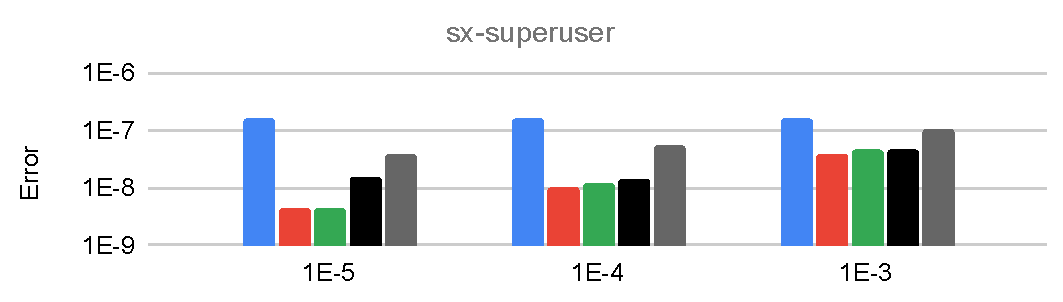
\includegraphics[width=0.48\linewidth]{out/temporal-summary-error-sx-superuser.pdf}
  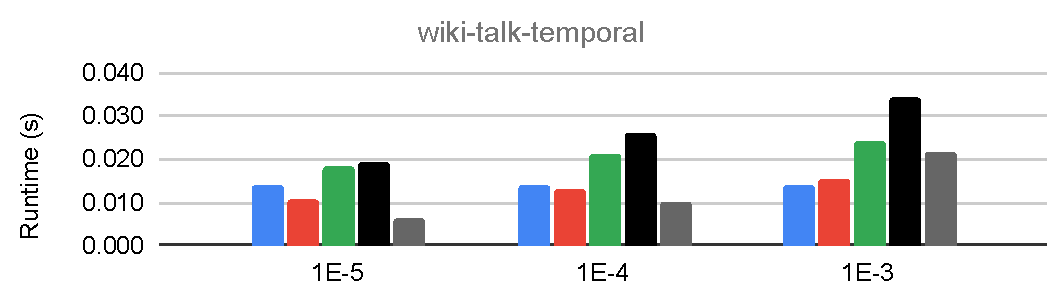
\includegraphics[width=0.48\linewidth]{out/temporal-summary-runtime-wiki-talk-temporal.pdf}
  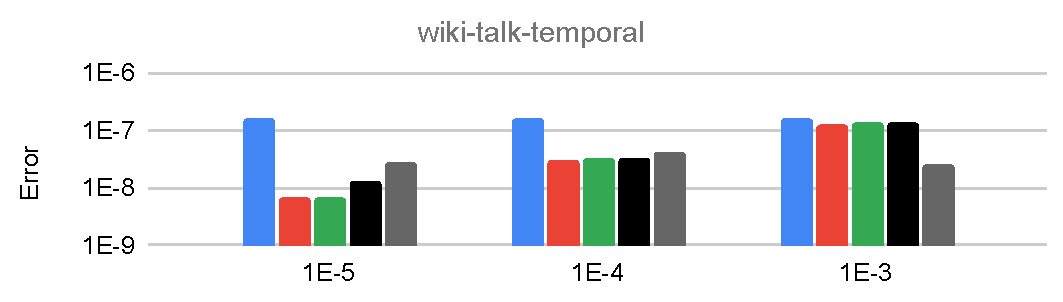
\includegraphics[width=0.48\linewidth]{out/temporal-summary-error-wiki-talk-temporal.pdf}
  \subfigure[Runtime on each dynamic graph]{
    \label{fig:temporal-summary--runtime-graph}
    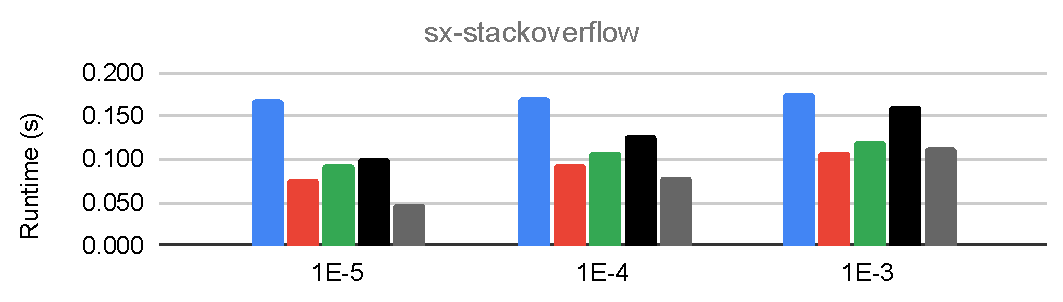
\includegraphics[width=0.48\linewidth]{out/temporal-summary-runtime-sx-stackoverflow.pdf}
  }
  \subfigure[Error in ranks obtained on each dynamic graph]{
    \label{fig:temporal-summary--error-graph}
    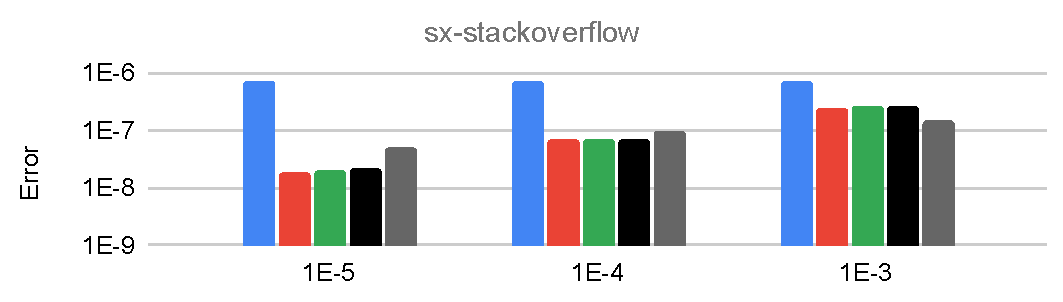
\includegraphics[width=0.48\linewidth]{out/temporal-summary-error-sx-stackoverflow.pdf}
  } \\[-2ex]
  \caption{Mean Runtime and Error in ranks obtained with \textit{Static}, \textit{Naive-dynamic (ND)}, \textit{Dynamic Traversal (DT)}, our improved \textit{Dynamic Frontier (DF)}, and our improved \textit{Dynamic Frontier with Pruning (DF-P)} PageRank on real-world dynamic graphs, with batch updates of size $10^{-5}|E_T|$ to $10^{-3}|E_T|$. Here, (a) and (b) show the overall runtime and error across all temporal graphs, while (c) and (d) show the runtime and rank error for each approach (relative to reference Static PageRank, see Section \ref{sec:measurement}). In (a), the speedup of each approach with respect to Static PageRank is labeled. \su{TOWR}}
  \label{fig:temporal-summary}
\end{figure*}

\begin{figure*}[hbtp]
  \centering
  \subfigure[Overall result]{
    \label{fig:8020-runtime--mean}
    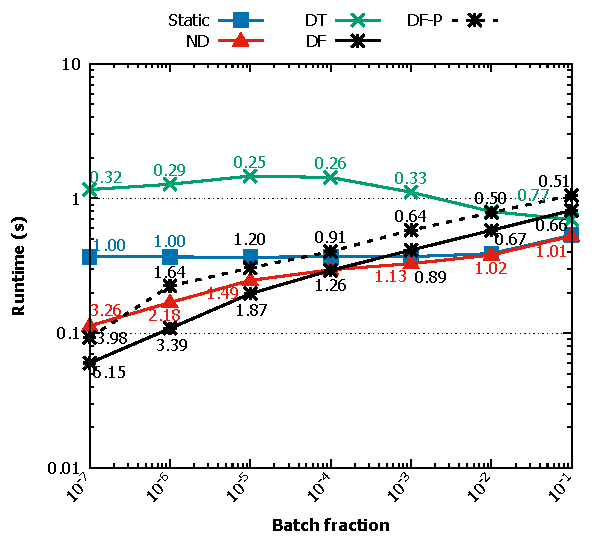
\includegraphics[width=0.38\linewidth]{out/8020-runtime-mean.pdf}
  }
  \subfigure[Results on each graph]{
    \label{fig:8020-runtime--all}
    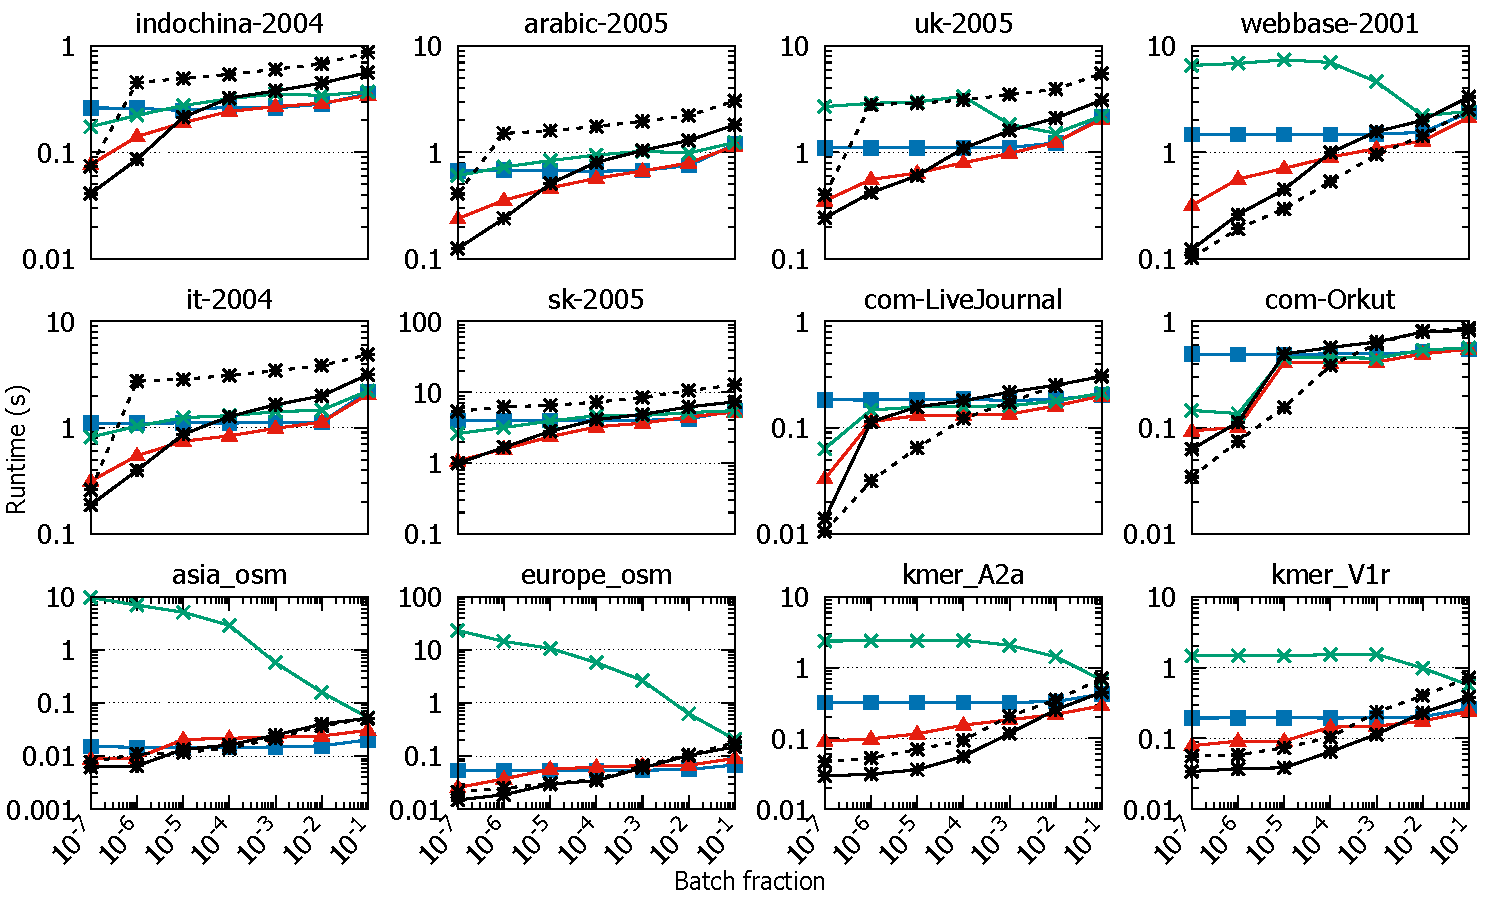
\includegraphics[width=0.58\linewidth]{out/8020-runtime-all.pdf}
  } \\[-1ex]
  \caption{Runtime (logarithmic scale) of GPU implementation for \textit{Static}, \textit{Naive-dynamic (ND)}, \textit{Dynamic Traversal (DT)}, our \textit{Dynamic Frontier (DF)}, and \textit{Dynamic Frontier with Pruning (DF-P)} PageRank on large (static) graphs with generated random batch updates. Batch updates range in size from $10^{-7}|E|$ to $0.1|E|$ in multiples of $10$. These updates consist of $80\%$ edge insertions and $20\%$ edge deletions, mimicking realistic changes in a dynamic graph scenario. The right subfigure illustrates the runtime of each approach for individual graphs in the dataset, while the left subfigure presents overall runtimes (using geometric mean for consistent scaling across graphs). Additionally, the speedup of each approach relative to Static PageRank is labeled\ignore{on respective lines}.}
  \label{fig:8020-runtime}
\end{figure*}

\begin{figure*}[hbtp]
  \centering
  \subfigure[Overall result]{
    \label{fig:8020-error--mean}
    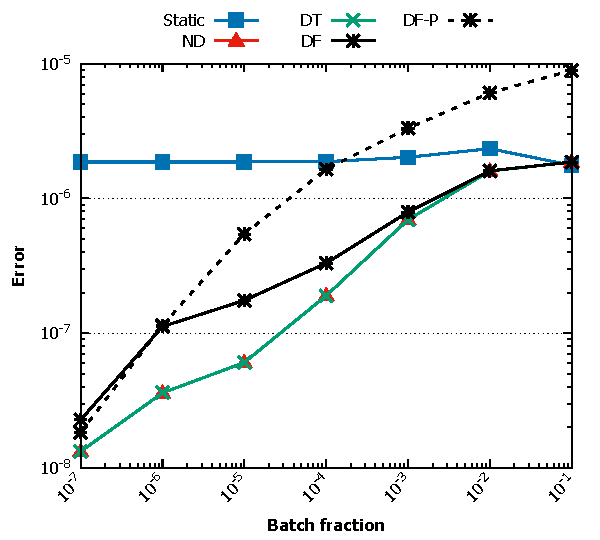
\includegraphics[width=0.38\linewidth]{out/8020-error-mean.pdf}
  }
  \subfigure[Results on each graph]{
    \label{fig:8020-error--all}
    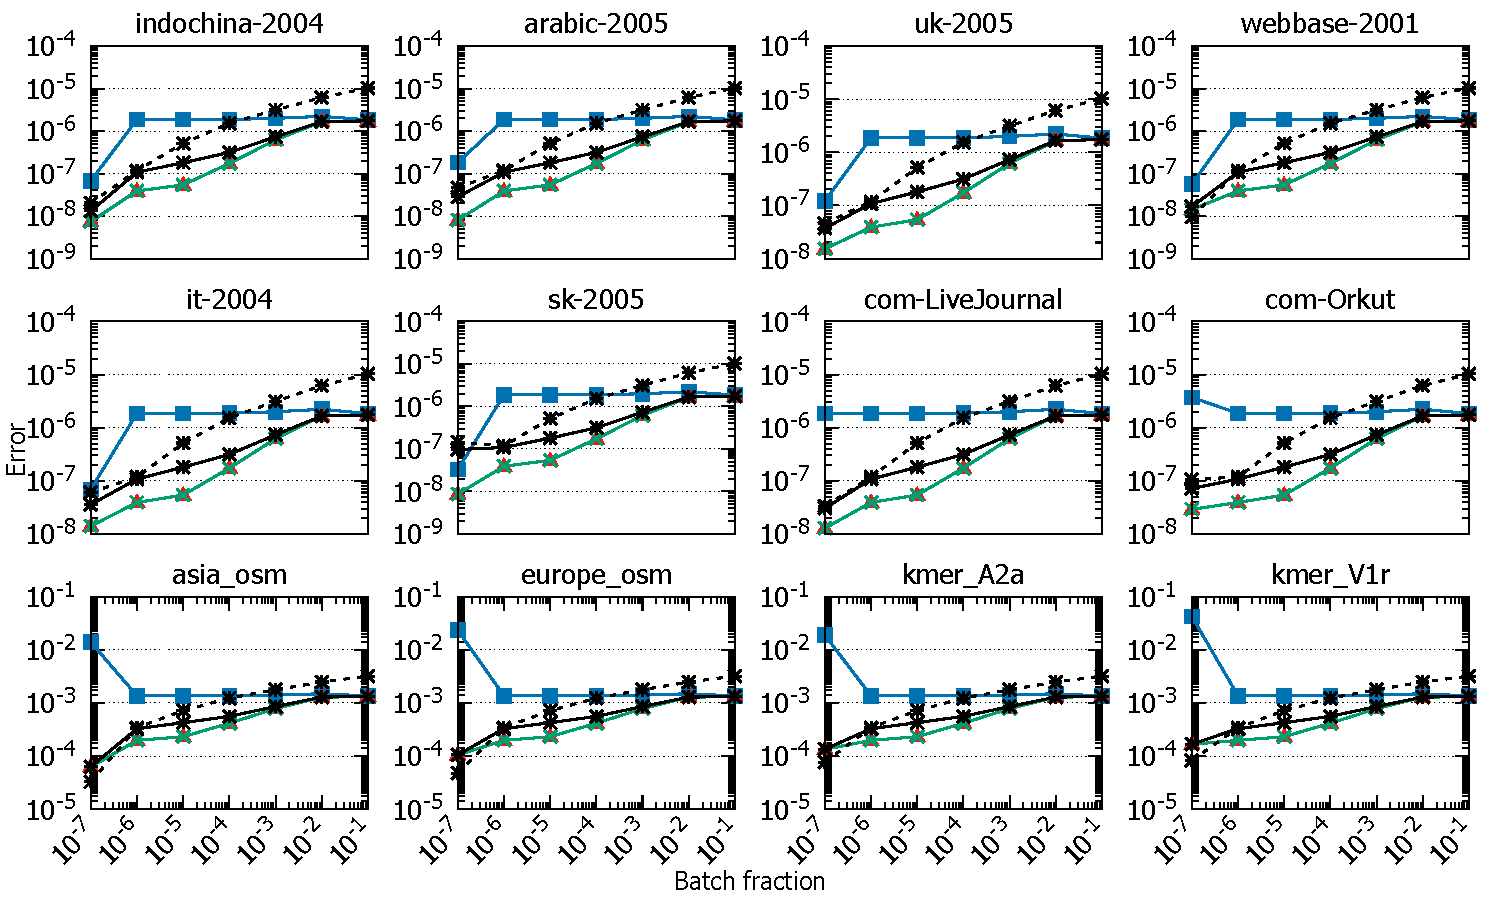
\includegraphics[width=0.58\linewidth]{out/8020-error-all.pdf}
  } \\[-1ex]
  \caption{Error comparison of our GPU implementation of \textit{Static}, \textit{Naive-dynamic (ND)}, \textit{Dynamic Traversal (DT)}, \textit{Dynamic Frontier (DF)}, and \textit{Dynamic Frontier with Pruning (DF-P)} PageRank on large (static) graphs with generated random batch updates, relative to a Reference Static PageRank (see Section \ref{sec:measurement}), using $L1$-norm. The size of batch updates range from $10^{-7} |E|$ to $0.1 |E|$ in multiples of $10$ (logarithmic scale), consisting of $80\%$ edge insertions and $20\%$ edge deletions to simulate realistic dynamic graph updates. The right subfigure depicts the error for each approach in relation to each graph, while the left subfigure showcases overall errors using geometric mean for consistent scaling across graphs.}
  \label{fig:8020-error}
\end{figure*}


Figure \ref{fig:temporal-summary--runtime-overall} shows that DF PageRank is, on average, $1.4\times$ faster than Static PageRank for batch updates of size $10^{-5}|E_T|$. In contrast, DF-P PageRank demonstrates average speedups of $3.6\times$, $2.0\times$, and $1.3\times$ over Static PageRank for batch update sizes of $10^{-5}|E_T|$, $10^{-4}|E_T|$, and $10^{-3}|E_T|$, respectively. Furthermore, DF-P PageRank achieves average speedups of $4.2\times$, $2.8\times$, and $3.6\times$ compared to DT PageRank for the same batch updates. This speedup is particularly pronounced on the \textit{sx-mathoverflow} graph, as indicated by Figure \ref{fig:temporal-summary--runtime-graph}. Regarding rank error, Figures \ref{fig:temporal-summary--error-overall} and \ref{fig:temporal-summary--error-graph} illustrate that DF and DF-P PageRank generally exhibit higher error on average compared to ND and DT PageRank but lower error than Static PageRank. This makes the ranks obtained with DF and DF-P PageRank acceptable. DF-P PageRank can thus be the default choice for updating PageRank scores on dynamic graphs. However, if elevated error levels are observed (during intermediate empirical tests), transitioning to ND PageRank is advisable.




\subsubsection{Results on large graphs with random updates}

We also assess the performance of our GPU implementation of DF and DF-P PageRank alongside Static, ND, and DT PageRank on large (static) graphs listed in Table \ref{tab:dataset-large}, with randomly generated batch updates. As elaborated in Section \ref{sec:batch-generation}, the batch updates vary in size from $10^{-7}|E|$ to $0.1|E|$ (in multiples of $10$), comprising $80\%$ edge insertions and $20\%$ edge deletions to mimic realistic scenarios. Self-loops are added to all vertices with each batch update. Figure \ref{fig:8020-runtime} illustrates the runtime of Static, ND, DT, DF, and DF-P PageRank, while Figure \ref{fig:8020-error} displays the error in ranks obtained with each approach. Figures \ref{fig:8020-runtime-compare} and \ref{fig:8020-error-compare} depict a comparison of the overall runtime and error between the GPU and CPU implementation of each approach.

Figure \ref{fig:8020-runtime--mean} illustrates that for batch updates ranging from $10^{-7}|E|$ to $10^{-4}|E|$, DF PageRank achieves an average speedup of $2.5\times$, $1.3\times$, and $10.4\times$ compared to Static, ND, and DT PageRank, respectively. Further, DF-P PageRank achieves average speedups of $3.1\times$, $1.7\times$, and $13.1\times$ over Static, ND, and DT PageRank, respectively. This acceleration is particularly pronounced on road networks and protein k-mer graphs, characterized by a low average degree (as depicted in Figure \ref{fig:8020-runtime--all}). It may be noted that DT PageRank exhibits slower performance than ND PageRank on large graphs with uniformly random batch updates. This is attributed to DT PageRank marking a significant number of vertices as affected, as updates are scattered randomly across the graph, rendering most of the graph reachable from the updated regions \cite{sahu2024incrementally}. Particularly on road networks and protein k-mer graphs, characterized by a low average degree and a large diameter, DT PageRank's performance is further hindered due to limited parallelism exploitable by the GPU. Figures \ref{fig:8020-error--mean} and \ref{fig:8020-error--all} indicate that DF-P PageRank generally exhibits higher error compared to ND, DT, and DF PageRank, but lower error than Static PageRank (up to a batch size of $10^{-4}|E|$). Hence, we recommend utilizing DF-P PageRank for large random batch updates up to a batch size of $10^{-4}|E|$. For larger batch updates, we advise the reader to switch to ND PageRank instead.


\ignore{\subsubsection{Comparison of vertices marked as affected}}

\ignore{Figure \ref{fig:measure-affected} displays the (mean) percentage of vertices marked as affected by Dynamic Traversal (DT), our improved Dynamic Frontier (DF), and Dynamic Frontier with Pruning (DF-P) PageRank on real-world dynamic graphs from Table \ref{tab:dataset}. This analysis is conducted on batch updates of size $10^{-5}|E_T|$ to $10^{-3}|E_T|$ in multiples of $10$ (see Section \ref{sec:batch-generation} for details). For DF and DF-P PageRank, affected vertices are marked incrementally --- therefore, we count all vertices that were ever flagged as affected.}

\ignore{As Figure \ref{fig:measure-affected} indicates, the proportion of vertices marked as affected by DF and DF-P PageRank is lower than DT PageRank for batch updates of size $10^{-5}|E_T|$, but comparable for larger batch updates. Therefore, the performance improvement with DF and DF-P PageRank is primarily attributed to the incremental marking of affected vertices. Additionally, it's worth noting that the percentage of vertices marked as affected is generally low across all approaches. This is likely because updates in real-world dynamic graphs tend to be concentrated in specific regions of the graph rather than being scattered throughout.}

\ignore{\begin{figure}[!hbt]
  \centering
  \subfigure{
    \label{fig:measure-affected--batch}
    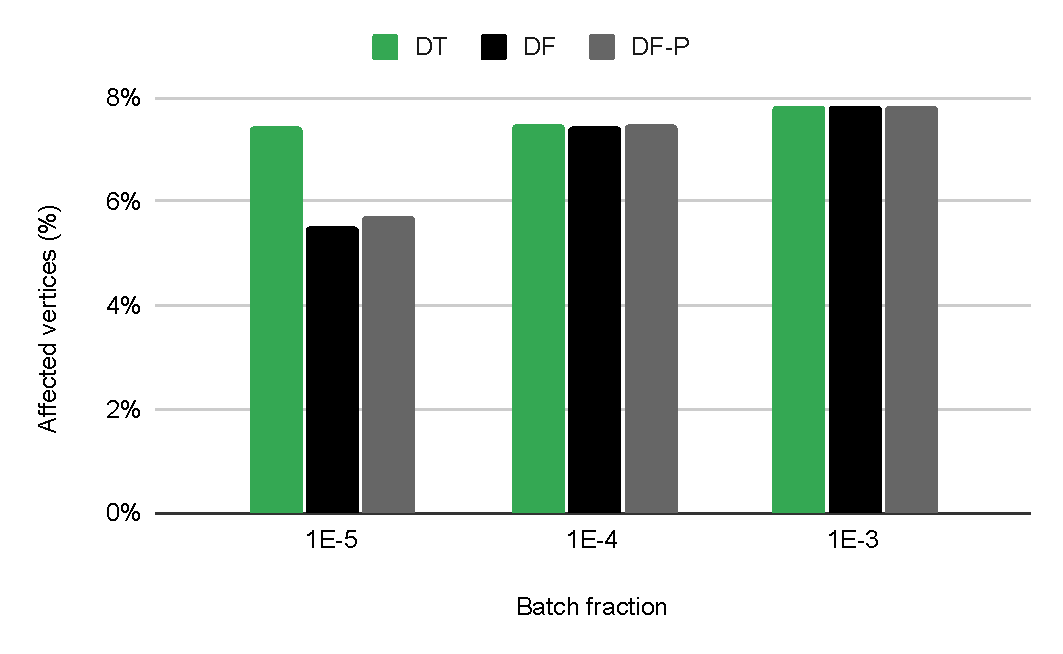
\includegraphics[width=0.98\linewidth]{out/measure-affected-batch.pdf}
  } \\[-2ex]
  \caption{Mean percentage of vertices marked as affected by \textit{Dynamic Traversal (DT)}, our improved \textit{Dynamic Frontier (DF)}, and \textit{Dynamic Frontier with Pruning (DF-P)} PageRank, on real-world graphs, with batch updates of size $10^{-5}|E_T|$ to $10^{-3}|E_T|$ (in multiples of $10$). DF and DF-P PageRank mark affected vertices incrementally --- thus, we count any vertex ever marked as affected. \su{TODO}}
  \label{fig:measure-affected}
\end{figure}
}
